
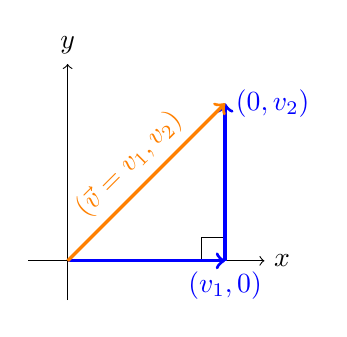
\begin{tikzpicture}
    %draw lines
    \draw [->] (-0.5,0) -- (2.5,0) node[right]{$x$};
    \draw [->] (0,-0.5) -- (0,2.5) node[above]{$y$};
    \draw [-] (1.7,0) -- (1.7,0.3);
    \draw [-] (1.7,0.3) -- (2,0.3);
    \draw [->,blue,very thick] (0,0) -- (2,0) node[below]{$(v_1,0)$};
    \draw [->,blue,very thick] (2,0) -- (2,2) node[right]{$(0,v_2)$};
    \draw [->,orange,very thick] (0,0) --  (2,2) node[midway,above,sloped]{$(\vec{v}=v_1,v_2)$};
\end{tikzpicture}
\captionof{figure}{{\footnotesize a vector $\vec{v}\in\mathbb{R}^2$}}
\label{fig:vector-and-vector-operation-d15}
